
\documentclass[letterpaper,hide notes,xcolor={table,svgnames},pdftex,10pt]{beamer}
\def\showexamples{t}


%\usepackage[svgnames]{xcolor}

%% Demo talk
%\documentclass[letterpaper,notes=show]{beamer}

\usecolortheme{crane}
\setbeamertemplate{navigation symbols}{}

\usetheme{MyPittsburgh}
%\usetheme{Frankfurt}

%\usepackage{tipa}

\usepackage{hyperref}
\usepackage{graphicx,xspace}
\usepackage[normalem]{ulem}
\usepackage{multicol}
\usepackage{amsmath,amssymb,amsthm,graphicx,xspace}
\newcommand\SF[1]{$\bigstar$\footnote{SF: #1}}

\usepackage[default]{sourcesanspro}
\usepackage[T1]{fontenc}
\usepackage[scaled]{beramono}
\usepackage{tikzpagenodes}

\newcounter{tmpnumSlide}
\newcounter{tmpnumNote}


% old question code
%\newcommand\question[1]{{$\bigstar$ \small \onlySlide{2}{#1}}}
% \newcommand\nquestion[1]{\ifdefined \presentationonly \textcircled{?} \fi \note{\par{\Large \textbf{?}} #1}}
% \newcommand\nanswer[1]{\note{\par{\Large \textbf{A}} #1}}


 \newcommand\mnote[1]{%
   \addtocounter{tmpnumSlide}{1}
   \ifdefined\showcues {~\tiny\fbox{\arabic{tmpnumSlide}}}\fi
   \note{\setlength{\parskip}{1ex}\addtocounter{tmpnumNote}{1}\textbf{\Large \arabic{tmpnumNote}:} {#1\par}}}

\newcommand\mmnote[1]{\note{\setlength{\parskip}{1ex}#1\par}}

%\newcommand\mnote[2][]{\ifdefined\handoutwithnotes {~\tiny\fbox{#1}}\fi
% \note{\setlength{\parskip}{1ex}\textbf{\Large #1:} #2\par}}

%\newcommand\mnote[2][]{{\tiny\fbox{#1}} \note{\setlength{\parskip}{1ex}\textbf{\Large #1:} #2\par}}

\newcommand\mquestion[2]{{~\color{red}\fbox{?}}\note{\setlength{\parskip}{1ex}\par{\Large \textbf{?}} #1} \note{\setlength{\parskip}{1ex}\par{\Large \textbf{A}} #2\par}\ifdefined \presentationonly \pause \fi}

\newcommand\blackboard[1]{%
\ifdefined   \showblackboard
  {#1}
  \else {\begin{center} \fbox{\colorbox{blue!30}{%
         \begin{minipage}{.95\linewidth}%
           \hspace{\stretch{1}} Some space intentionally left blank; done at the blackboard.%
         \end{minipage}}}\end{center}}%
         \fi%
}



%\newcommand\q{\tikz \node[thick,color=black,shape=circle]{?};}
%\newcommand\q{\ifdefined \presentationonly \textcircled{?} \fi}

\usepackage{listings}
\lstset{basicstyle=\footnotesize\ttfamily,
	breaklines=true,
	aboveskip=15pt,
  	belowskip=15pt,
	frame=lines,
	numbers=left, basicstyle=\scriptsize, numberstyle=\tiny, stepnumber=0, numbersep=2pt
}

\usepackage{siunitx}
\newcommand\sius[1]{\num[group-separator = {,}]{#1}\si{\micro\second}}
\newcommand\sims[1]{\num[group-separator = {,}]{#1}\si{\milli\second}}
\newcommand\sins[1]{\num[group-separator = {,}]{#1}\si{\nano\second}}
\sisetup{group-separator = {,}, group-digits = true}

%% -------------------- tikz --------------------
\usepackage{tikz}
\usetikzlibrary{positioning}
\usetikzlibrary{arrows,backgrounds,automata,decorations.shapes,decorations.pathmorphing,decorations.markings,decorations.text,decorations.pathreplacing}

\tikzstyle{place}=[circle,draw=blue!50,fill=blue!20,thick, inner sep=0pt,minimum size=6mm]
\tikzstyle{transition}=[rectangle,draw=black!50,fill=black!20,thick, inner sep=0pt,minimum size=4mm]

\tikzstyle{block}=[rectangle,draw=black, thick, inner sep=5pt]
\tikzstyle{bullet}=[circle,draw=black, fill=black, thin, inner sep=2pt]

\tikzstyle{pre}=[<-,shorten <=1pt,>=stealth',semithick]
\tikzstyle{post}=[->,shorten >=1pt,>=stealth',semithick]
\tikzstyle{bi}=[<->,shorten >=1pt,shorten <=1pt, >=stealth',semithick]

\tikzstyle{mut}=[-,>=stealth',semithick]

\tikzstyle{treereset}=[dashed,->, shorten >=1pt,>=stealth',thin]

\usepackage{ifmtarg}
\usepackage{xifthen}
\makeatletter
% new counter to now which frame it is within the sequence
\newcounter{multiframecounter}
% initialize buffer for previously used frame title
\gdef\lastframetitle{\textit{undefined}}
% new environment for a multi-frame
\newenvironment{multiframe}[1][]{%
\ifthenelse{\isempty{#1}}{%
% if no frame title was set via optional parameter,
% only increase sequence counter by 1
\addtocounter{multiframecounter}{1}%
}{%
% new frame title has been provided, thus
% reset sequence counter to 1 and buffer frame title for later use
\setcounter{multiframecounter}{1}%
\gdef\lastframetitle{#1}%
}%
% start conventional frame environment and
% automatically set frame title followed by sequence counter
\begin{frame}%
\frametitle{\lastframetitle~{\normalfont(\arabic{multiframecounter})}}%
}{%
\end{frame}%
}
\makeatother

\makeatletter
\newdimen\tu@tmpa%
\newdimen\ydiffl%
\newdimen\xdiffl%
\newcommand\ydiff[2]{%
    \coordinate (tmpnamea) at (#1);%
    \coordinate (tmpnameb) at (#2);%
    \pgfextracty{\tu@tmpa}{\pgfpointanchor{tmpnamea}{center}}%
    \pgfextracty{\ydiffl}{\pgfpointanchor{tmpnameb}{center}}%
    \advance\ydiffl by -\tu@tmpa%
}
\newcommand\xdiff[2]{%
    \coordinate (tmpnamea) at (#1);%
    \coordinate (tmpnameb) at (#2);%
    \pgfextractx{\tu@tmpa}{\pgfpointanchor{tmpnamea}{center}}%
    \pgfextractx{\xdiffl}{\pgfpointanchor{tmpnameb}{center}}%
    \advance\xdiffl by -\tu@tmpa%
}
\makeatother
\newcommand{\copyrightbox}[3][r]{%
\begin{tikzpicture}%
\node[inner sep=0pt,minimum size=2em](ciimage){#2};
\usefont{OT1}{phv}{n}{n}\fontsize{4}{4}\selectfont
\ydiff{ciimage.south}{ciimage.north}
\xdiff{ciimage.west}{ciimage.east}
\ifthenelse{\equal{#1}{r}}{%
\node[inner sep=0pt,right=1ex of ciimage.south east,anchor=north west,rotate=90]%
{\raggedleft\color{black!50}\parbox{\the\ydiffl}{\raggedright{}#3}};%
}{%
\ifthenelse{\equal{#1}{l}}{%
\node[inner sep=0pt,right=1ex of ciimage.south west,anchor=south west,rotate=90]%
{\raggedleft\color{black!50}\parbox{\the\ydiffl}{\raggedright{}#3}};%
}{%
\node[inner sep=0pt,below=1ex of ciimage.south west,anchor=north west]%
{\raggedleft\color{black!50}\parbox{\the\xdiffl}{\raggedright{}#3}};%
}
}
\end{tikzpicture}
}


%% --------------------

%\usepackage[excludeor]{everyhook}
%\PushPreHook{par}{\setbox0=\lastbox\llap{MUH}}\box0}

%\vspace*{\stretch{1}

%\setbox0=\lastbox \llap{\textbullet\enskip}\box0}

\setlength{\parskip}{\fill}

\newcommand\noskips{\setlength{\parskip}{1ex}}
\newcommand\doskips{\setlength{\parskip}{\fill}}

\newcommand\xx{\par\vspace*{\stretch{1}}\par}
\newcommand\xxs{\par\vspace*{2ex}\par}
\newcommand\tuple[1]{\langle #1 \rangle}
\newcommand\code[1]{{\sf \footnotesize #1}}
\newcommand\ex[1]{\uline{Example:} \ifdefined \presentationonly \pause \fi
  \ifdefined\showexamples#1\xspace\else{\uline{\hspace*{2cm}}}\fi}

\newcommand\ceil[1]{\lceil #1 \rceil}


\AtBeginSection[]
{
   \begin{frame}
       \frametitle{Outline}
       \tableofcontents[currentsection]
   \end{frame}
}



\pgfdeclarelayer{edgelayer}
\pgfdeclarelayer{nodelayer}
\pgfsetlayers{edgelayer,nodelayer,main}

\tikzstyle{none}=[inner sep=0pt]
\tikzstyle{rn}=[circle,fill=Red,draw=Black,line width=0.8 pt]
\tikzstyle{gn}=[circle,fill=Lime,draw=Black,line width=0.8 pt]
\tikzstyle{yn}=[circle,fill=Yellow,draw=Black,line width=0.8 pt]
\tikzstyle{empty}=[circle,fill=White,draw=Black]
\tikzstyle{bw} = [rectangle, draw, fill=blue!20, 
    text width=4em, text centered, rounded corners, minimum height=2em]
    
    \newcommand{\CcNote}[1]{% longname
	This work is licensed under the \textit{Creative Commons #1 3.0 License}.%
}
\newcommand{\CcImageBy}[1]{%
	\includegraphics[scale=#1]{creative_commons/cc_by_30.pdf}%
}
\newcommand{\CcImageSa}[1]{%
	\includegraphics[scale=#1]{creative_commons/cc_sa_30.pdf}%
}
\newcommand{\CcImageNc}[1]{%
	\includegraphics[scale=#1]{creative_commons/cc_nc_30.pdf}%
}
\newcommand{\CcGroupBySa}[2]{% zoom, gap
	\CcImageBy{#1}\hspace*{#2}\CcImageNc{#1}\hspace*{#2}\CcImageSa{#1}%
}
\newcommand{\CcLongnameByNcSa}{Attribution-NonCommercial-ShareAlike}

\newenvironment{changemargin}[1]{% 
  \begin{list}{}{% 
    \setlength{\topsep}{0pt}% 
    \setlength{\leftmargin}{#1}% 
    \setlength{\rightmargin}{1em}
    \setlength{\listparindent}{\parindent}% 
    \setlength{\itemindent}{\parindent}% 
    \setlength{\parsep}{\parskip}% 
  }% 
  \item[]}{\end{list}} 




\title{Lecture 10 --- Of Asgard and Hel }

\author{Jeff Zarnett \& Patrick Lam \\ \small \texttt{jzarnett@uwaterloo.ca, patrick.lam@uwaterloo.ca}}
\institute{Department of Electrical and Computer Engineering \\
  University of Waterloo}
\date{\today}


\begin{document}

\begin{frame}
  \titlepage

 \end{frame}

\begin{frame}
\frametitle{Ginnungagap}

\begin{center}
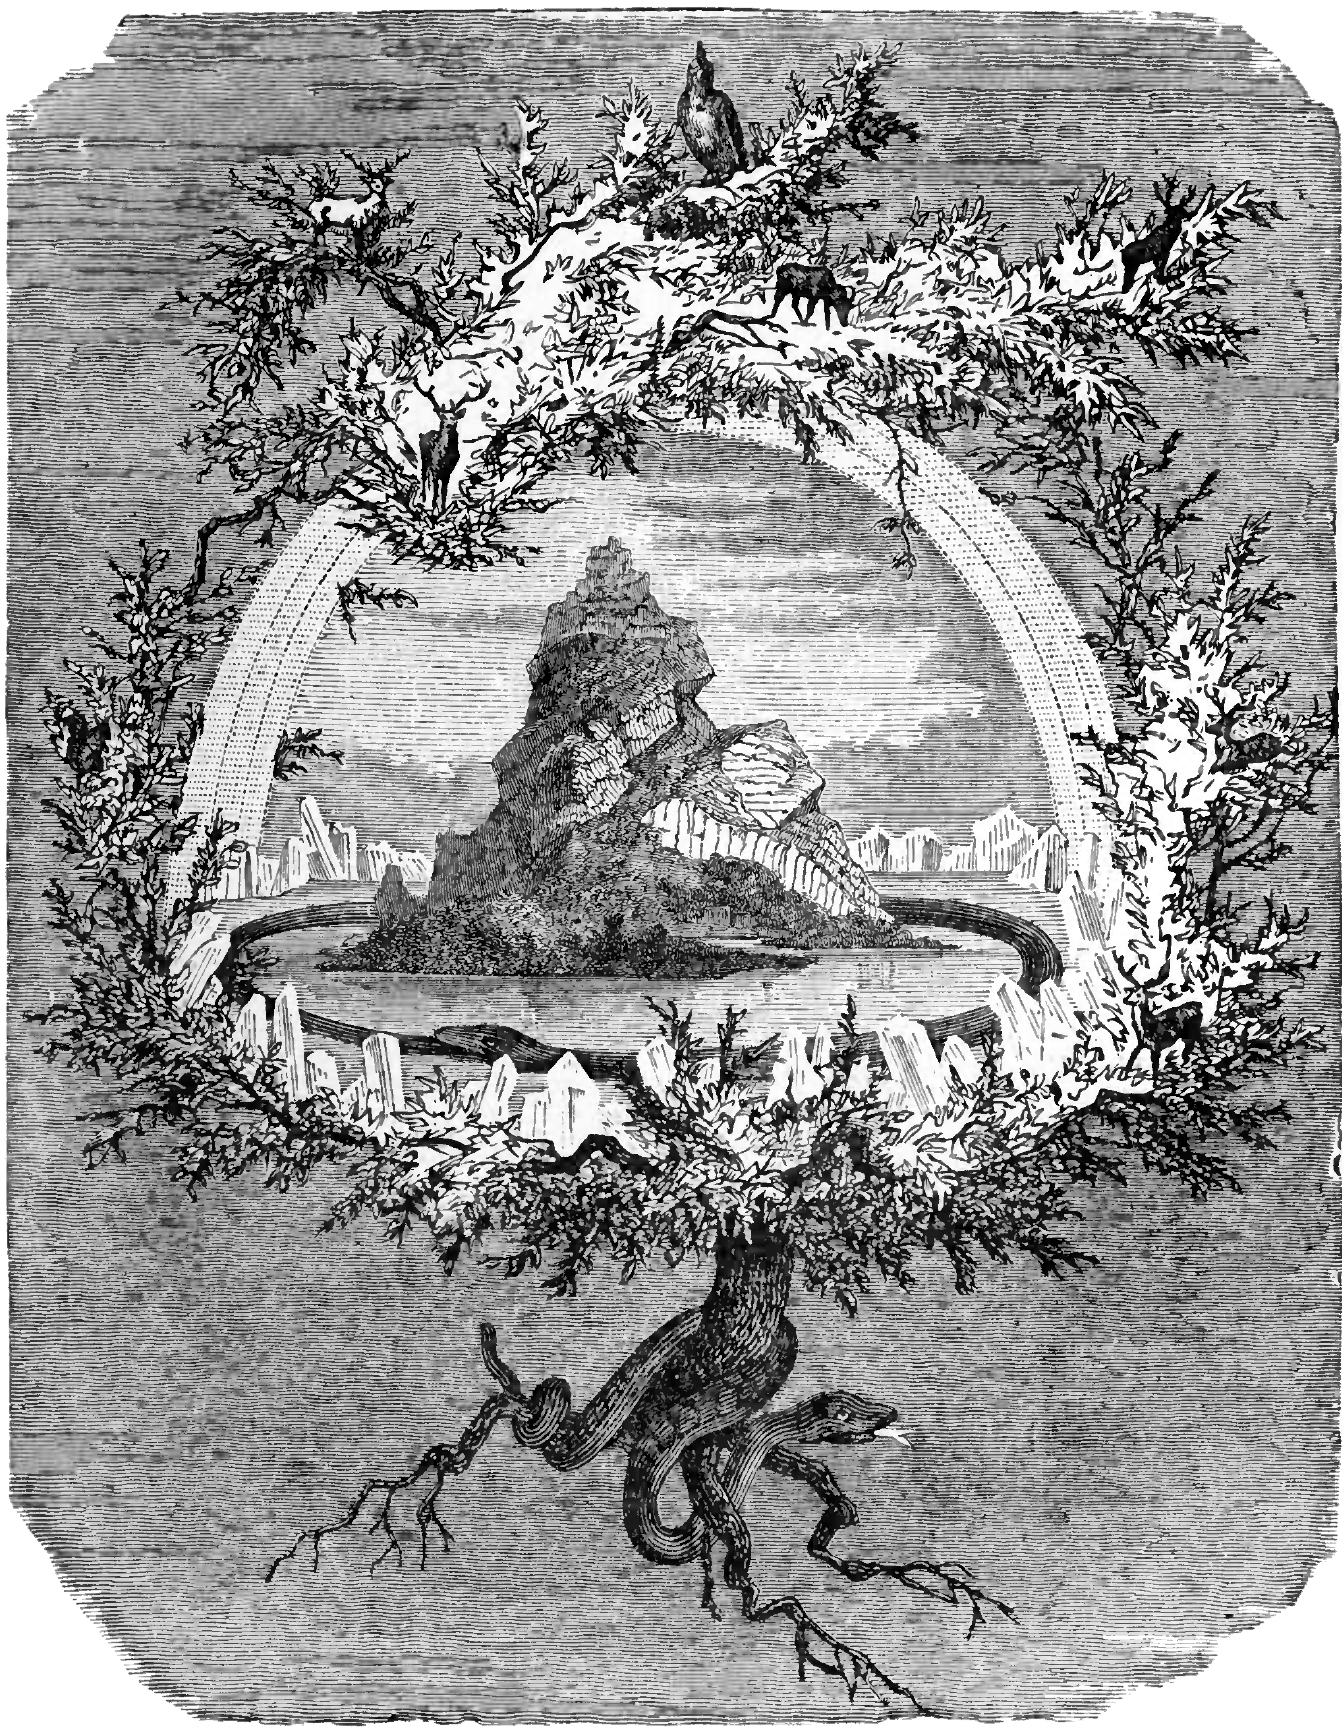
\includegraphics[height=.8\textheight]{images/L10-yggdrasil.jpg}

``The Ash Yggdrasil'' (1886) by Friedrich Wilhelm Heine, \\
courtesy Wikimedia Commons.
\end{center}

%% Everything came into creation in the gap between fire and ice, and the World Tree (Yggdrasil) connects the nine worlds. 

%% Asgard is the home of the \AE sir, the Norse gods. 

%% Helheim, or simply Hel, is the underworld where the dead go upon their death. 

%%  In Hel or Asgard (it's not clear), there is Valhalla, hall of the honoured dead. 

\end{frame}

\begin{frame}[fragile]
\frametitle{The Nine Worlds}
\Large
\url{http://riordan.wikia.com/wiki/File:Magnus_Chase_NINE_WORLDS_Target.jpg}
\end{frame}

\begin{frame}
\frametitle{Carry We, Who Die In Battle\ldots}

\begin{center}
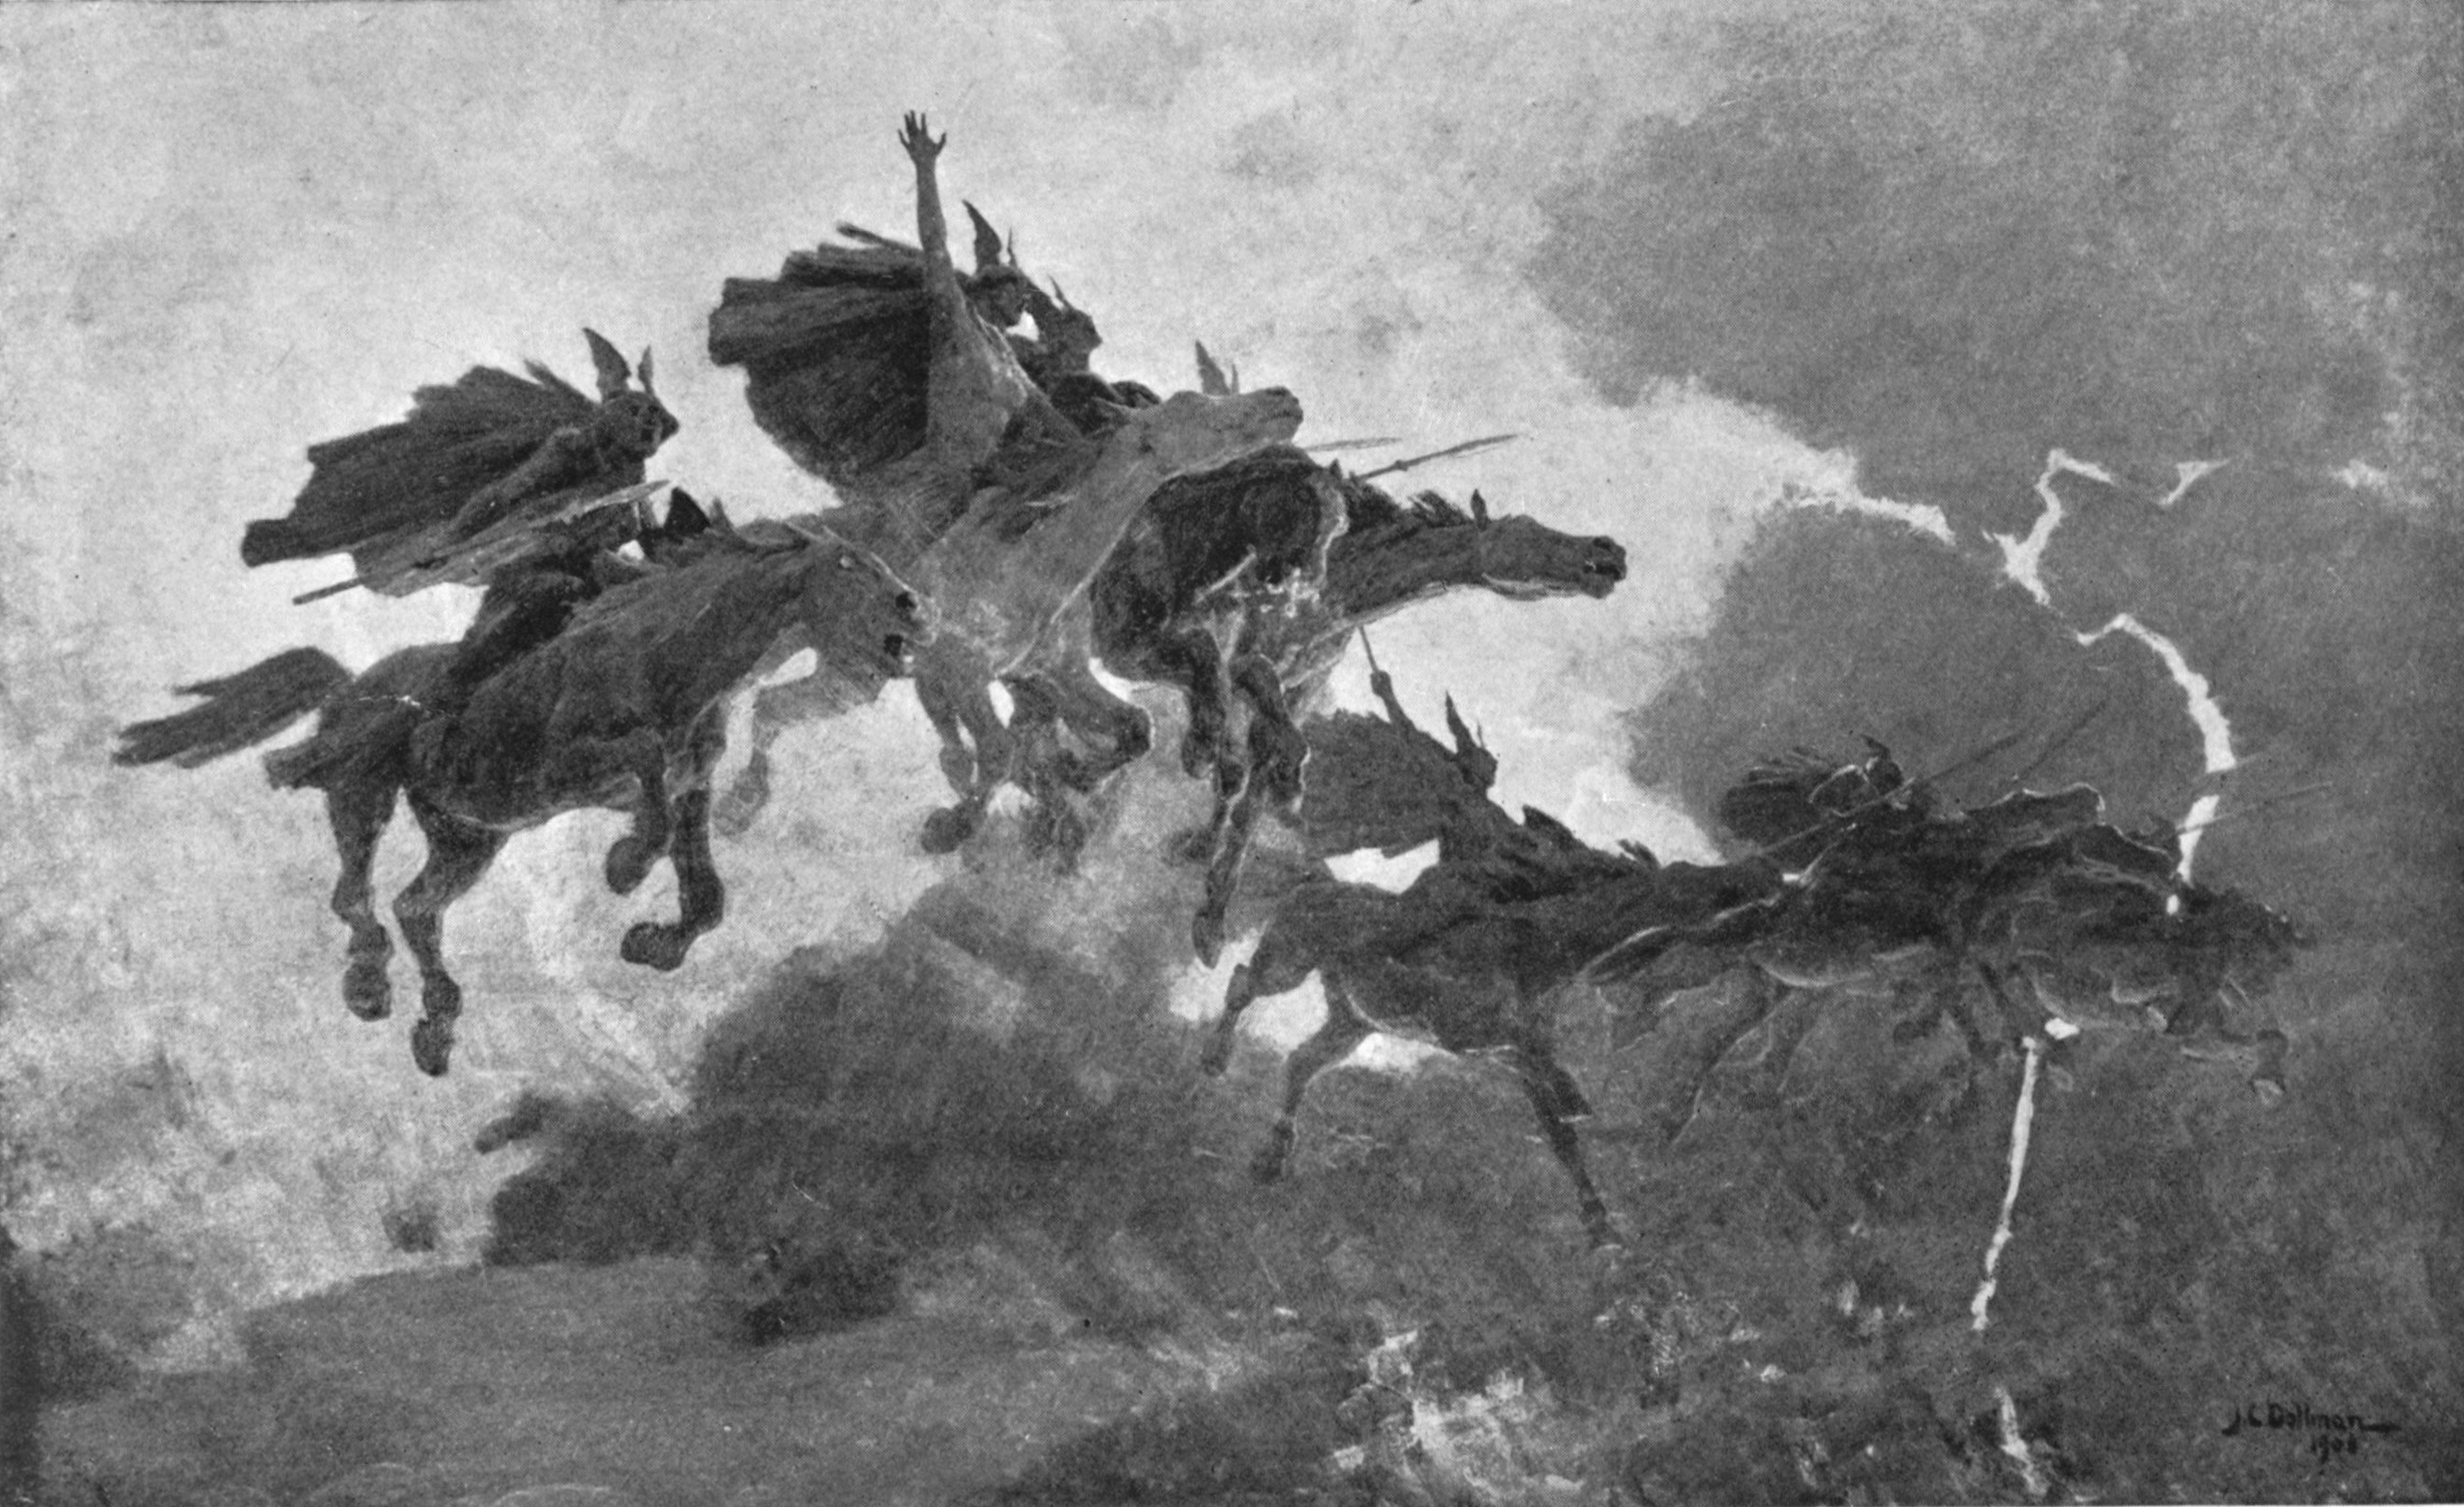
\includegraphics[height=.8\textheight]{images/L10-ride-of-the-valkyrs.jpg}

``The Ride of the Valkyrs'' (1909) by John Charles Dollman, \\
courtesy Wikimedia Commons.
\end{center}
\end{frame}

\begin{frame}
\frametitle{Boss fight\ldots}

\begin{center}
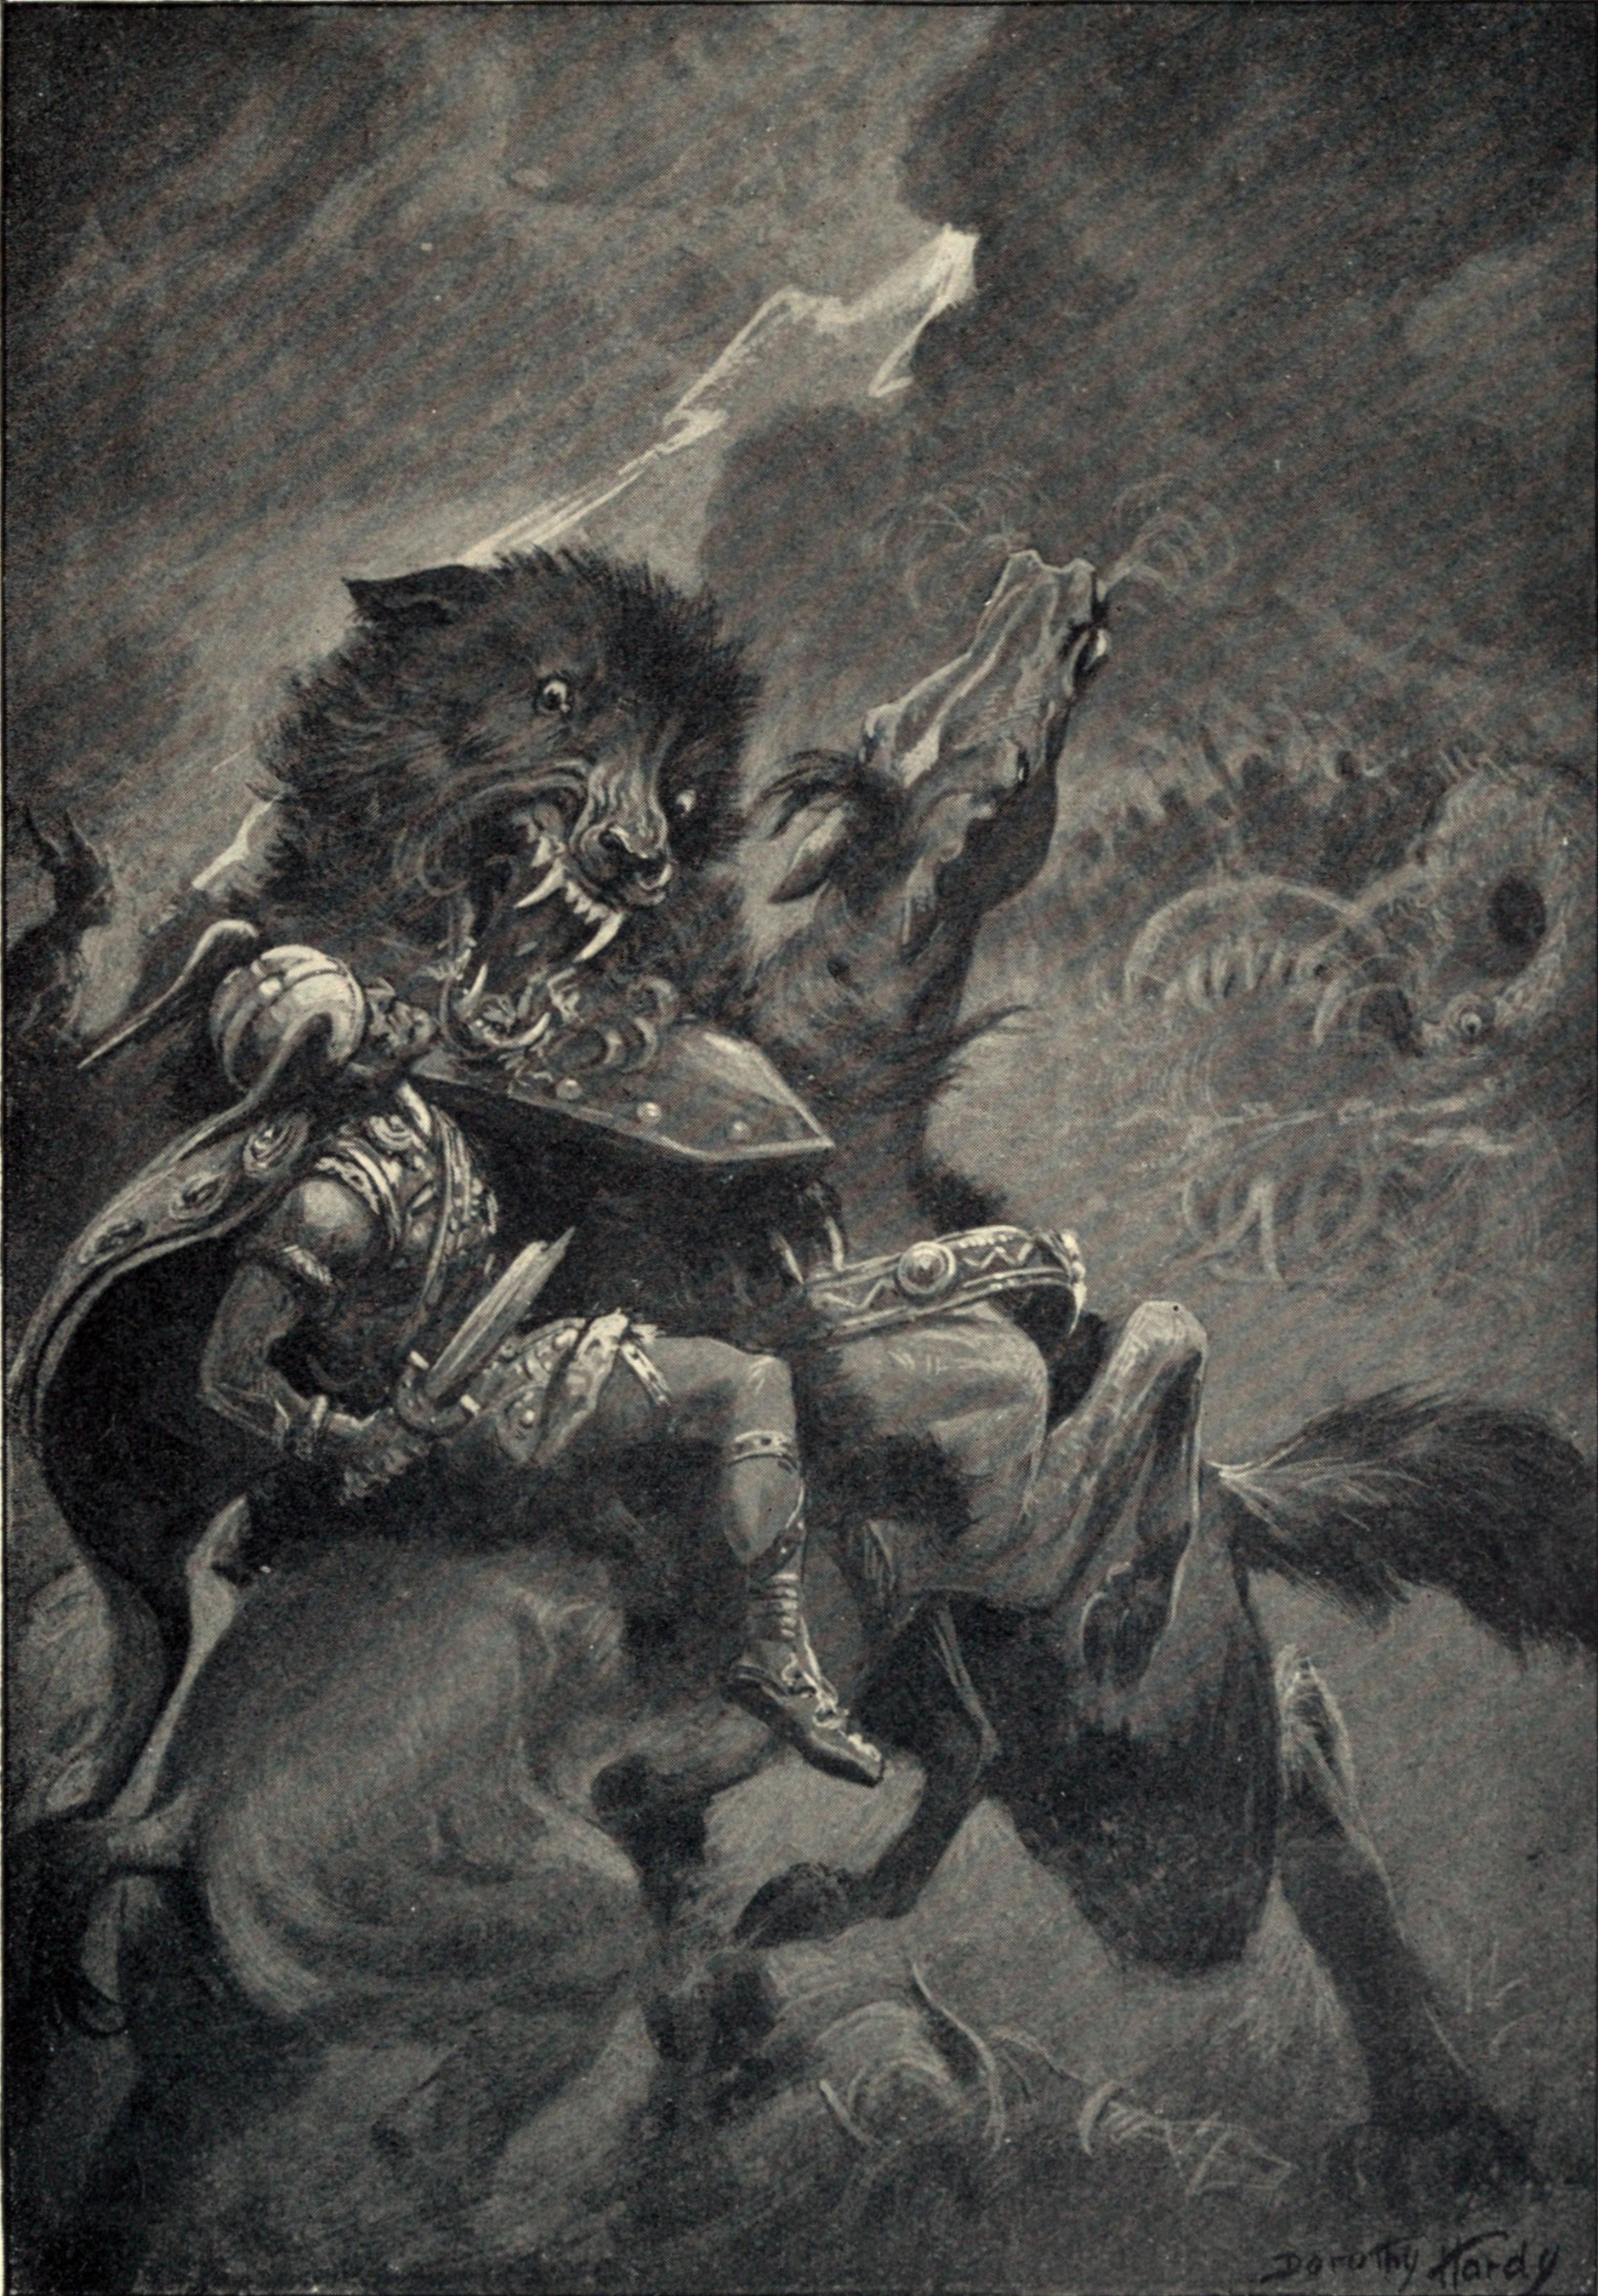
\includegraphics[height=.8\textheight]{images/L10-odin-and-fenris.jpg}

``Odin and Fenris'' (1909) by Dorothy Hardy, \\
courtesy Wikipedia
\end{center}
\end{frame}

%% Those who die in battle and are judged worthy will be carried to Valhalla by the Valkyries. 

%% There they will reside until they are called upon to aid in Odin's fight with the wolf Fenrir in Ragnar\"ok.

%% humans live in the ``middle realm'', Midg\aa rd, surrounded by the serpent Jormungand, who will fight against Thor in  Ragnar\"ok. 

%% Thor will kill the serpent, but the serpent's poison will also finish off Thor.


\begin{frame}
\frametitle{Across the Rainbow Bridge, To Valhalla...}


\tikzstyle{bt} = [rectangle, draw, fill=blue!20, 
    text width=4em, text centered, rounded corners, minimum height=2em]

\begin{center}
\begin{tikzpicture}[->,>=stealth',shorten >=1pt,auto,node distance=2cm,
                    semithick,initial text=]
  \node[bt]   (m) {Midgard};
  \node[bt, below of=m]   (hel) {Hel};
  \node[bt, left of=m, xshift=-5em]   (val) {Valhalla};

  \path (m) edge node[right] {Helgrind} (hel)
  (m) edge node[above] {Valgrind} (val);
\end{tikzpicture}
\end{center}

[\Large]
Cachegrind? Not so much.

%% We're going to examine some very useful tools for programming called Valgrind and Helgrind (also Cachegrind).

%% Where do they take their names from? Valgrind is the gateway to Valhalla; a gate that only the worthy can pass. 

%% Helgrind is the gateway to, well, Hel. 

%%  Sadly, the authors of Cachegrind failed to choose a name that corresponds to a location in the nine worlds of Norse mythology. 

\end{frame}

\begin{frame}
\frametitle{Through the Bifrost}

All of these are analysis tools for your C and C++ programs. 

They are absolute murder on performance, but they are wonderful for finding errors in your program. 

To use them, start the tool of your choice and instruct it to invoke your program. 

The target program then runs under the ``supervision'' of the tool.

Remember to enable debugging symbols in your compile.

\end{frame}

\begin{frame}
\frametitle{Valgrind (memcheck)}

Valgrind is the base name of the project and by default what it's going to do is run the memcheck tool. 

The purpose of memcheck is to look into all memory reads, writes, and to intercept and analyze every call to \texttt{malloc}/\texttt{free} and \texttt{new}/\texttt{delete}.

\end{frame}

\begin{frame}
\frametitle{Is Your Program Worthy?}

Memcheck can find problems like:
\begin{itemize}
	\item Accessing uninitialized memory
	\item Reading off the end of an array
	\item Memory leaks
	\item Incorrect freeing of memory
	\item Incorrect use of C standard functions like \texttt{memcpy}
	\item Using memory after it's been freed.
	\item Asking for an invalid number of bytes in an allocation
\end{itemize}

\end{frame}

\begin{frame}[fragile]
\frametitle{Valgrind Output}
{\scriptsize
\begin{verbatim}
jz@Loki:~/ece254$ valgrind ./search
==8476== Memcheck, a memory error detector
==8476== Copyright (C) 2002-2013, and GNU GPL'd, by Julian Seward et al.
==8476== Using Valgrind-3.10.0.SVN and LibVEX; rerun with -h for copyright info
==8476== Command: /usr/local/bin/search
==8476== 
usage: search [arguments] [options]
arguments:
         for text
         in directory
options:
         -c | --case-sensitive
         -s | --show-filenames-only
==8476== 
==8476== HEAP SUMMARY:
==8476==     in use at exit: 0 bytes in 0 blocks
==8476==   total heap usage: 0 allocs, 0 frees, 0 bytes allocated
==8476== 
==8476== All heap blocks were freed -- no leaks are possible
==8476== 
==8476== For counts of detected and suppressed errors, rerun with: -v
==8476== ERROR SUMMARY: 0 errors from 0 contexts (suppressed: 0 from 0)
\end{verbatim}
}

\end{frame}

\begin{frame}
\frametitle{No, It's Because I'm Awesome}

Okay, everything going perfectly is unlikely in anything other than a small program. 

The exam question I used this on is something like 62 lines (including blanks). 

So it's a trivial program. But I'll sabotage it a bit so we get a more interesting result. 

Suppose I delete from the code two of the \texttt{free()} calls.

\end{frame}

\begin{frame}[fragile]
\frametitle{Hence the word... Sabotage}
{\scriptsize
\begin{verbatim}
jz@Loki:~/ece254$ valgrind ./search 
==8678== Memcheck, a memory error detector
==8678== Copyright (C) 2002-2013, and GNU GPL'd, by Julian Seward et al.
==8678== Using Valgrind-3.10.0.SVN and LibVEX; rerun with -h for copyright info
==8678== Command: ./search
==8678== 
Found at 11 by thread 1 
Found at 22 by thread 3 
==8678== 
==8678== HEAP SUMMARY:
==8678==     in use at exit: 1,614 bytes in 4 blocks
==8678==   total heap usage: 17 allocs, 13 frees, 2,822 bytes allocated
==8678== 
==8678== LEAK SUMMARY:
==8678==    definitely lost: 0 bytes in 0 blocks
==8678==    indirectly lost: 0 bytes in 0 blocks
==8678==      possibly lost: 0 bytes in 0 blocks
==8678==    still reachable: 1,614 bytes in 4 blocks
==8678==         suppressed: 0 bytes in 0 blocks
==8678== Rerun with --leak-check=full to see details of leaked memory
==8678== 
==8678== For counts of detected and suppressed errors, rerun with: -v
==8678== ERROR SUMMARY: 0 errors from 0 contexts (suppressed: 0 from 0)
\end{verbatim}
}

\end{frame}


\begin{frame}
\frametitle{Send the Plumbers to the Watergate}


Take the program's suggestion to use the \texttt{--leak-check=full}.

You get a bit more detail about where you made the mistake. 

In the example below, lines 49 and 24 in the file \texttt{search.c} are the locations of the \texttt{malloc} calls that lack a matching call to \texttt{free}. 

It can't tell you where the call to \texttt{free} should go, only where the memory that isn't freed was allocated.

\end{frame}

\begin{frame}[fragile]
\frametitle{Fixing the Leaks}

{\scriptsize
\begin{verbatim}
==8553== 16 bytes in 4 blocks are definitely lost in loss record 1 of 2
==8553==    at 0x4C2AB80: malloc (in /usr/lib/valgrind/vgpreload_memcheck-amd64-linux.so)
==8553==    by 0x40084D: search (search.c:49)
==8553==    by 0x4E3F181: start_thread (pthread_create.c:312)
==8553==    by 0x514F47C: clone (clone.S:111)
==8553== 
==8553== 48 bytes in 4 blocks are definitely lost in loss record 2 of 2
==8553==    at 0x4C2AB80: malloc (in /usr/lib/valgrind/vgpreload_memcheck-amd64-linux.so)
==8553==    by 0x40074E: main (search.c:24)
\end{verbatim}
}

\end{frame}

\begin{frame}[fragile]
\frametitle{Not My Problem!}

But it's also important to learn what to ignore. 

I decided to deploy Valgrind on the solution to the producer-consumer problem from ECE~254 and I ended up with a result that says:

\begin{verbatim}
==8734==      possibly lost: 544 bytes in 2 blocks
\end{verbatim}

Hmm. Let's dig into that with the \texttt{--leak-check=full} option:

\end{frame}

\begin{frame}[fragile]
\frametitle{Ignore and Continue}
{\scriptsize
\begin{verbatim}
==8734== 272 bytes in 1 blocks are possibly lost in loss record 1 of 2
==8734==    at 0x4C2CC70: calloc (in /usr/lib/valgrind/vgpreload_memcheck-amd64-linux.so)
==8734==    by 0x4012E54: _dl_allocate_tls (dl-tls.c:296)
==8734==    by 0x4E3FDA0: pthread_create@@GLIBC_2.2.5 (allocatestack.c:589)
==8734==    by 0x400A57: main (mutex.c:64)
\end{verbatim}
}

Looking in the file, at that line, we see a call to \texttt{pthread\_create} and this is therefore probably nothing we need to do anything about. 


\end{frame}

\begin{frame}
\frametitle{Reading the Output}

\begin{itemize}
	\item \textbf{Definitely lost}
	\item \textbf{Indirectly lost}
	\item \textbf{Possibly lost}
	\item \textbf{Still reachable}
	\item \textbf{Suppressed}
\end{itemize}



\end{frame}

\begin{frame}
\frametitle{What Fresh Hel is This}

The purpose of Helgrind is to detect errors in the use of POSIX pthreads. 

In a way, Helgrind is a pretty neat tool for improving performance, even though it doesn't actually directly speed anything up. 

When we take single-threaded program and split it off into a multithreaded program, we may introduce a lot of errors.

Humans are not very good at parallel thinking; we are very much sequential.

\end{frame}

\begin{frame}
\frametitle{What Fresh Hel is This}

But a program that is fast and wrong is probably less useful than one that is slow and correct. 

But can we make it faster and still have it be correct? 

That's the goal of Helgrind: determine where, if anywhere, there are concurrency problems. 

It can't prove that your program is correct (if only) but it can at least catch some of the common problems you might introduce when writing a parallel program.

\end{frame}

\begin{frame}
\frametitle{Hel Hath No Fury...}

Helgrind puts errors into three basic categories:

\begin{enumerate}
	\item Misuses of the pthreads API
	\item Lock ordering problems
	\item Data races
\end{enumerate}


\end{frame}

\begin{frame}
\frametitle{Misuse of the API}

The first category does not require much explanation:


\begin{itemize}
	\item Unlocking a mutex that is unlocked
	\item Deallocation of memory with a locked mutex in it
	\item Thread exit while holding a locked lock
\end{itemize}
... and many more.


\end{frame}

\begin{frame}[fragile]
\frametitle{API Misuse Error Output}


\begin{verbatim}
Thread #1 unlocked a not-locked lock at 0x7FEFFFA90
   at 0x4C2408D: pthread_mutex_unlock (hg_intercepts.c:492)
   by 0x40073A: nearly_main (tc09_bad_unlock.c:27)
   by 0x40079B: main (tc09_bad_unlock.c:50)
  Lock at 0x7FEFFFA90 was first observed
   at 0x4C25D01: pthread_mutex_init (hg_intercepts.c:326)
   by 0x40071F: nearly_main (tc09_bad_unlock.c:23)
   by 0x40079B: main (tc09_bad_unlock.c:50)
\end{verbatim}

\end{frame}

\begin{frame}[fragile]
\frametitle{Type Two Errors}

The second category of errors should be familiar to you:

\begin{multicols}{2}
\textbf{Thread P}
  \begin{verbatim}
	 1. wait( a ) 
	 2. wait( b )
	 3. [critical section]
	 4. signal( a )
	 5. signal( b )
  \end{verbatim}
\columnbreak
\textbf{Thread Q}
  \begin{verbatim}
	 1. wait( b ) 
	 2. wait( a )
	 3. [critical section]
	 4. signal( b )
	 5. signal( a )
  \end{verbatim}
\end{multicols}
\vspace{-2em}

Potential Deadlock!

\end{frame}

\begin{frame}
\frametitle{Interleaving Leaves Locks}

Risk of deadlock: thread P holds mutex \texttt{a} and thread Q holds mutex \texttt{b}. 

Each waits for the mutex that the other one has. 

The example is slightly silly, of course, because it's super easy to see. 

There will not necessarily be an obvious (alphabetical) order.

\end{frame}

\begin{frame}
\frametitle{Graph Theory Strikes Back}


Helgrind builds a directed graph of lock acquisitions, so that when a thread acquires a lock, the graph is checked to see if a cycle exists. 

  It will report as an error the initial order (the first order seen is the one viewed as ``correct'') and the the ``incorrect'' order that is the source of the potential problem. 
  
  Really, though, all that matters is consistency.

\end{frame}

\begin{frame}[fragile]
\frametitle{Order of a Mutex Lock}
{\scriptsize
\begin{verbatim}
Thread #1: lock order "0x7FF0006D0 before 0x7FF0006A0" violated

Observed (incorrect) order is: acquisition of lock at 0x7FF0006A0
   at 0x4C2BC62: pthread_mutex_lock (hg_intercepts.c:494)
   by 0x400825: main (tc13_laog1.c:23)

 followed by a later acquisition of lock at 0x7FF0006D0
   at 0x4C2BC62: pthread_mutex_lock (hg_intercepts.c:494)
   by 0x400853: main (tc13_laog1.c:24)

Required order was established by acquisition of lock at 0x7FF0006D0
   at 0x4C2BC62: pthread_mutex_lock (hg_intercepts.c:494)
   by 0x40076D: main (tc13_laog1.c:17)

 followed by a later acquisition of lock at 0x7FF0006A0
   at 0x4C2BC62: pthread_mutex_lock (hg_intercepts.c:494)
   by 0x40079B: main (tc13_laog1.c:18)
\end{verbatim}
}

\end{frame}

\begin{frame}
\frametitle{Category 3}

The third category we have discussed already.

  Recall the earlier definition of a race condition. 

 Helgrind looks for when two threads access the same memory location without using locks.

\end{frame}

\begin{frame}[fragile]
\frametitle{It's a Race!}
{\scriptsize
\begin{verbatim}
jz@Loki:~/ece459$ valgrind --tool=helgrind ./datarace
==10389== Helgrind, a thread error detector
==10389== Copyright (C) 2007-2013, and GNU GPL'd, by OpenWorks LLP et al.
==10389== Using Valgrind-3.10.0.SVN and LibVEX; rerun with -h for copyright info
==10389== Command: ./datarace
==10389== 
==10389== ---Thread-Announcement------------------------------------------
==10389== 
==10389== Thread #1 is the program's root thread
==10389== 
==10389== ---Thread-Announcement------------------------------------------
==10389== 
==10389== Thread #2 was created
==10389==    at 0x515543E: clone (clone.S:74)
==10389==    by 0x4E44199: do_clone.constprop.3 (createthread.c:75)
==10389==    by 0x4E458BA: pthread_create@@GLIBC_2.2.5 (createthread.c:245)
==10389==    by 0x4C30C90: ??? (in /usr/lib/valgrind/vgpreload_helgrind-amd64-linux.so)
==10389==    by 0x40068D: main (datarace.c:12)
==10389== 
==10389== ----------------------------------------------------------------
\end{verbatim}
}

\end{frame}

\begin{frame}[fragile]
\frametitle{It's a Race}
{\scriptsize
\begin{verbatim}
==10389== Possible data race during read of size 4 at 0x60104C by thread #1
==10389== Locks held: none
==10389==    at 0x40068E: main (datarace.c:13)
==10389== 
==10389== This conflicts with a previous write of size 4 by thread #2
==10389== Locks held: none
==10389==    at 0x40065E: child_fn (datarace.c:6)
==10389==    by 0x4C30E26: ??? (in /usr/lib/valgrind/vgpreload_helgrind-amd64-linux.so)
==10389==    by 0x4E45181: start_thread (pthread_create.c:312)
==10389==    by 0x515547C: clone (clone.S:111)
==10389== 
==10389== ----------------------------------------------------------------
==10389== 
==10389== Possible data race during write of size 4 at 0x60104C by thread #1
==10389== Locks held: none
==10389==    at 0x400697: main (datarace.c:13)
==10389== 
==10389== This conflicts with a previous write of size 4 by thread #2
==10389== Locks held: none
==10389==    at 0x40065E: child_fn (datarace.c:6)
==10389==    by 0x4C30E26: ??? (in /usr/lib/valgrind/vgpreload_helgrind-amd64-linux.so)
==10389==    by 0x4E45181: start_thread (pthread_create.c:312)
==10389==    by 0x515547C: clone (clone.S:111)
\end{verbatim}
}
\end{frame}

\begin{frame}
\frametitle{Always Two, There Are}


Note that we get two stack traces here: we have a read after write, and a write after write. 

Why? 

Because the operation in question is \texttt{var++} which necessitates fetching the current value of \texttt{var} (reading it) and incrementing it (then writing it back).

\end{frame}

\begin{frame}
\frametitle{Behind the Scenes}

It examines the use of the standard threading primitives - lock, unlock, signal/post, wait... 

Anything that implies there might be an ordering between events is taken and added to a directed acyclic graph that represents these dependencies. 

If memory is accessed from two different threads and there is no path through this directed acyclic graph that indicates an ordering, then a race is reported. 

Although obviously at least one of these accesses must be a write.

\end{frame}

\begin{frame}[fragile]
\frametitle{Name \& Shame}

You can ask Helgrind to try to tell you about variable names (if it can) with the command line option \texttt{--read-var-info=yes}.

\begin{verbatim}
==10454== Location 0x60104c is 0 bytes inside global var "var"
==10454== declared at datarace.c:3
\end{verbatim}

\end{frame}

\begin{frame}
\frametitle{Fixing it Isn't My Problem}


The authors of Helgrind assume that if it tells you where the problem is, you will figure out what variables are affected and how to properly prevent data races. 

You might find this frustrating. 


Helgrind + OpenMP + Linux can cause the occasional problem in GCC 4.2 and 4.3; the ``futex'' system call in Linux is not visible to Helgrind. 

You can rebuild GCC with the option \texttt{--disable-linux-futex} and that will hopefully work it out.


\end{frame}

\begin{frame}
\frametitle{Cachegrind}

This is much more performance oriented than the other two tools. 

 It runs a simulation of how your program interacts with cache and evaluates how your program does on branch prediction.
 
 As we discussed earlier, cache misses and branch mispredicts have a huge impact on performance.
 
 Recall that a miss from the fastest cache results in a small penalty (10 cycles).
 
 A miss that requires going to memory requires about 200 cycles. 
 
 A mispredicted branch costs somewhere between 10-30 cycles.


\end{frame}

\begin{frame}
\frametitle{Cachegrind Reporting}

Cachegrind reports data about:
\begin{itemize}
	\item The First Level Instruction Cache (I1) [L1 Instruction Cache]
	\item The First Level Data Cache (D1) [L1 Data Cache]
	\item The Last Level Cache (LL) [L3 Cache].
\end{itemize}

Unlike normal Valgrind operation, you probably want to turn optimizations on.

\end{frame}

\begin{frame}[fragile]
\frametitle{Sim-u-laaaaate!}
{\scriptsize

\begin{verbatim}
jz@Loki:~/ece254$ valgrind --tool=cachegrind --branch-sim=yes ./search

--16559-- warning: L3 cache found, using its data for the LL simulation.
Found at 11 by thread 1 
Found at 22 by thread 3 
==16559== 
==16559== I   refs:      310,670
==16559== I1  misses:      1,700
==16559== LLi misses:      1,292
==16559== I1  miss rate:    0.54%
==16559== LLi miss rate:    0.41%
==16559== 
==16559== D   refs:      114,078  (77,789 rd   + 36,289 wr)
==16559== D1  misses:      4,398  ( 3,360 rd   +  1,038 wr)
==16559== LLd misses:      3,252  ( 2,337 rd   +    915 wr)
==16559== D1  miss rate:     3.8% (   4.3%     +    2.8%  )
==16559== LLd miss rate:     2.8% (   3.0%     +    2.5%  )
==16559== 
==16559== LL refs:         6,098  ( 5,060 rd   +  1,038 wr)
==16559== LL misses:       4,544  ( 3,629 rd   +    915 wr)
==16559== LL miss rate:      1.0% (   0.9%     +    2.5%  )
==16559== 
==16559== Branches:       66,622  (65,097 cond +  1,525 ind)
==16559== Mispredicts:     7,202  ( 6,699 cond +    503 ind)
==16559== Mispred rate:     10.8% (  10.2%     +   32.9%   )

\end{verbatim}
}

\end{frame}

\begin{frame}[fragile]
\frametitle{Optimizations: Enabled!}
{\scriptsize
\begin{verbatim}
jz@Loki:~/ece254$ valgrind --tool=cachegrind --branch-sim=yes ./search

--16618-- warning: L3 cache found, using its data for the LL simulation.
Found at 11 by thread 1 
Found at 22 by thread 3 
==16618== 
==16618== I   refs:      306,169
==16618== I1  misses:      1,652
==16618== LLi misses:      1,286
==16618== I1  miss rate:    0.53%
==16618== LLi miss rate:    0.42%
==16618== 
==16618== D   refs:      112,015  (76,522 rd   + 35,493 wr)
==16618== D1  misses:      4,328  ( 3,353 rd   +    975 wr)
==16618== LLd misses:      3,201  ( 2,337 rd   +    864 wr)
==16618== D1  miss rate:     3.8% (   4.3%     +    2.7%  )
==16618== LLd miss rate:     2.8% (   3.0%     +    2.4%  )
==16618== 
==16618== LL refs:         5,980  ( 5,005 rd   +    975 wr)
==16618== LL misses:       4,487  ( 3,623 rd   +    864 wr)
==16618== LL miss rate:      1.0% (   0.9%     +    2.4%  )
==16618== 
==16618== Branches:       65,827  (64,352 cond +  1,475 ind)
==16618== Mispredicts:     7,109  ( 6,596 cond +    513 ind)
==16618== Mispred rate:     10.7% (  10.2%     +   34.7%   )
\end{verbatim}
}

\end{frame}

\begin{frame}
\frametitle{Results Analysis}


Interesting results: our data and instruction miss rates went down marginally but the branch mispredict rates went up!

Well sort of - there were fewer branches and thus fewer we got wrong as well as fewer we got right. 

So the total cycles lost to mispredicts went down. 

Is this an overall win for the code? Yes. 


\end{frame}
\begin{frame}
\frametitle{Do the Math}

In some cases it's not so clear cut, and we could do a small calculation. 

If we just take a look at the LL misses (4~544 vs 4~487) and assume they take 200 cycles, and the branch miss penalty is 200 cycles, it went from 908~800 wasted cycles to 897~400. This is a decrease of 11~400 cycles.

  Repeat for each of the measures and sum them up to determine if things got better overall and by how much.

\end{frame}
\begin{frame}
\frametitle{Cachegrind Detailed Output}

Cachegrind also produces a more detailed output file, titled cachegrind.out.<pid> (the PID in the example is 16618). 

This file is not especially human-readable, but we can ask the associated tool \texttt{cg\_annotate} to break it down for us.

The output is way too big for slides.

\end{frame}
\begin{frame}
\frametitle{Advanced Cachegrind}

Cachegrind is very... verbose... and it can be very hard to come up with useful changes based on what you see... 

Assuming your eyes don't glaze over when you see the numbers. 

Probably the biggest performance impact is last level cache misses (those appear as DLmr or DLmw). 

You might also try to look at the Bcm and Bim (branch mispredictions) to see if you can give some better hints. 
\end{frame}
\begin{frame}
\frametitle{Really Advanced Cachegrind}

Of course, to learn more about how Cachegrind, the manual is worth reading. 

Not that anybody reads manuals anymore... 

Just give it a shot, when you get stuck, google the problem, click the first stack overflow link result...


\end{frame}

\end{document}

